\documentclass{beamer}
\input{../style/cours-style.sty}

% Title
\title[JavaScript]{JavaScript Frontend - B1 Web et Multimédia}
\author{Christophe Brun}
\institute{My Digital School}
\beamertemplatenavigationsymbolsempty

\titlegraphic{
    \bigbreak
    
\includegraphics[width=5cm]{image/mds-logo}
    \bigbreak
    L’école des métiers du digital
    \bigbreak
}

\begin{document}

    \begin{frame}
        \titlepage
        \bigbreak
        \centering
        \url{https://github.com/My-Digital-School-by-PapIT/frontend-JS}
    \end{frame}


    \section{Table des matières}\label{sec:toc}

    \begin{frame}{Table des matières}
        \begin{tiny}
            \begin{multicols}{1}
                \tableofcontents
            \end{multicols}
        \end{tiny}
    \end{frame}


    \section{Programme du module}\label{sec:programme-du-module}

    \begin{frame}{JavaScript Frontend}{Objectifs des 6 jours}
        \begin{columns}
            \column{0.7\textwidth}
            \begin{scriptsize}
                \begin{itemize}
                    \item Distinguer les différentes parties prenantes du web (protocol de communication, navigateur, serveur, \textit{etc}).
                    \item La syntaxe JavaScript.
                    \item La Window API, manipulation de DOM.
                    \item Intéragir avec une API depuis le frontend.
                \end{itemize}
            \end{scriptsize}
            \column{0.3\textwidth}
            
\includegraphics[width=4cm]{image/js-surfing}
        \end{columns}
    \end{frame}


    \section{Introduction}\label{sec:introduction}

    \begin{frame}{Formateur sur Linux}{Christophe Brun, conseil en développement informatique}

        \begin{columns}
            \column{0.7\textwidth}
            \begin{itemize}
                \item Développeur freelance (Python, Java, CoBOL) et data at scale.

                \item 7 ans de conseil en développement au sein d'SSII~.

                \item 7 ans de conseil en développement en indépendant, \href{https://papit.fr}{PapIT}.

                \item Passionné~!
                \bigbreak
                \begin{columns}
                    \column{0.5\textwidth}
                    \centering
                    
\includegraphics[width=3cm]{image/logo-uppa}
                    \column{0.5\textwidth}
                    \centering
                    
\includegraphics[width=3cm]{image/logo-universite-bordeaux}
                \end{columns}
            \end{itemize}
            \column{0.3\textwidth}
            \centering
            
\includegraphics[width=5cm]{image/trombine-christophe}
        \end{columns}
    \end{frame}


    \section{Les ressources du Web}\label{sec:ressources}

    \begin{frame}{Les ressources du Web}{Dvisions en briques}
        \begin{columns}
            \column{0.6\textwidth}
            1 des 4 règles pour la direction de l'esprit de Descartes~: \textquote{Diviser chacune des difficultés que j'examinerais, en autant de parcelles qu'il se pourrait et qu'il serait requis pour les mieux résoudre.}.
            \column{0.4\textwidth}
            \centering
            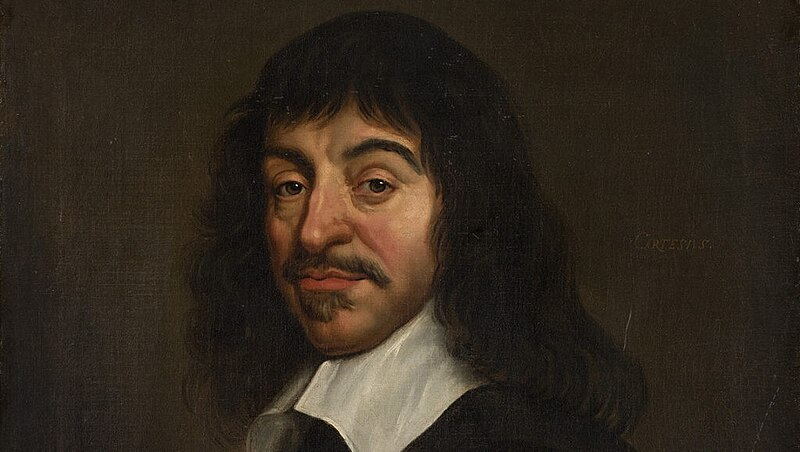
\includegraphics[width=6cm]{image/Descartes}
        \end{columns}
    \end{frame}

    \begin{frame}{Les ressources du Web}{Analyse des composants}
        \centering
        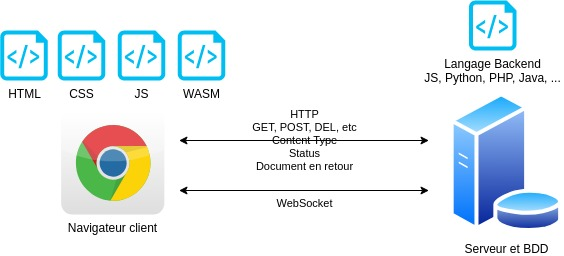
\includegraphics[width=11cm]{image/web-stakeholders.drawio}
    \end{frame}


    \section{Le web statique}\label{sec:static}

    \begin{frame}{Le web statique}
        Une des premières options pour un site web est donc d'être statique.

        Suite à une requête sur une URL (adresse dans le navigateur), le serveur nous envoie une page HTML pour la donnée avec du CSS pour le style.
        \bigbreak
        Il n'y a pas d'interaction avec le serveur, le contenu est figé, on peut juste passer à une autre page grâce à une ancre \lstinline{<a href="...">...</a>}.
        \bigbreak
        \centering
        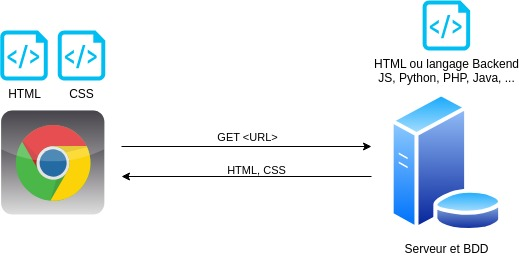
\includegraphics[width=8cm]{image/web-static}
    \end{frame}

    \begin{frame}[fragile]{Développement Web Statique}{Exercice \execcounterdispinc{}}
        \begin{itemize}
            \item Installer Python 3.
            \item Installer un IDE de développement Web comme WebStorm.
            \item Lancer un serveur HTTP avec la commande dans le répertoire du cours~:
            \begin{lstlisting}[language=bash]
python3 -m http.server
            \end{lstlisting}
            \item Naviguer à l'adresse indiquée.
            \item Modifier le fichier \lstinline{index.html} pour ajouter un lien vers une page HTML développée par vos soins avec votre nom et une photo de vous.
            \item Rafraîchir la page et vérifier que la modification est fonctionnelle.
        \end{itemize}
    \end{frame}


    \section{Le web dynamique}\label{sec:Dynamic}
    \begin{frame}{Développement Web Dynamique}{Exercice \execcounterdispinc{}}
        \begin{itemize}
            \item Quelles seraient les moyens d'avoir des pages web dynamiques~?
        \end{itemize}
        \bigbreak
        \centering
        
\includegraphics[width=5cm]{image/question-mark}
    \end{frame}

    \begin{frame}{Développement Web Dynamique}{Backend}
        Un serveur qui fait tourner un algorithme qui sert des données qui évoluent (dans la base de données), ou de l'extérieur (API).

        Plusieurs requêtes sont nécessaires, de différents types~:
        \begin{itemize}
            \item Des GET comme auparavant pour retourner des données.
            \item Des POST pour envoyer des données au serveur.
            \item Des DEL pour supprimer des données de la base de données du serveur.
        \end{itemize}
        \bigbreak
        \centering
        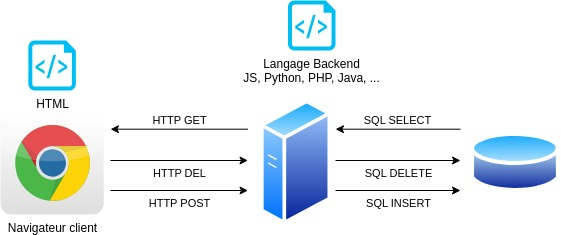
\includegraphics[width=7cm]{image/web-dynamic-backend}
    \end{frame}

    \begin{frame}{Frontend}
        \begin{small}
            Il est également possible de modifier une page web sans recharger la page entière, en utilisant JavaScript.

            Le JavaScript est un des langages qui peuvent être interprétés par le navigateur.

            Ces langages sont~:
            \begin{itemize}
                \item \textbf{HTML}, un langage de balisage, à l'image du XML, c'est le document principal de la page.
                Il peut contenir de la mise en forme, des données à afficher, \textit{etc}.
                \item \textbf{CSS}, un langage de style, qui permet de définir la mise en forme de la page.
                C'est une manière \textbf{modulaire} de définir le style de tout un site web.
                \item \textbf{JavaScript}, un langage de programmation qui permet de modifier le contenu de la page sans recharger la page.
                Il peut modifier~:
                \begin{itemize}
                    \item Le contenu de la page, ses données (DOM API\footnotemark{}).
                    \item Le style de la page, la mise en forme (DOM API\cref{DOM}).
                    \item Intéragir avec n'importe quel serveur.
                \end{itemize}
            \end{itemize}
        \end{small}
        \footnotetext{\label{DOM}DOM (Document Object Model), \url{https://developer.mozilla.org/fr/docs/Glossary/DOM}}
    \end{frame}


    \section{Généralité sur le JavaScript en Frontend}\label{sec:js-basic}

    \subsection{Où est-il~?}\label{sec:where}

    \begin{frame}{Où se trouve le JavaScript ?}
        Deux solutions, ils se trouvent~:
        \begin{itemize}
            \item Dans le fichier HTML, entre les balises \lstinline{<script>...</script>}.
            \item Dans un fichier séparé, avec l'attribut \lstinline{src} de la balise \lstinline{<script>} qui indique le chemin de ce fichier.
            Comme le fichier de style, cette méthode est plus modulaire, car ce fichier peut être partagé entre plusieurs pages.
        \end{itemize}
        \bigbreak
        \begin{dangercolorbox}
            En programmation, être modulaire est une importante qualité. Si on réutilise, on est écrit moins.
            Ici, dans un seul fichier.
            Si on écrit moins, on écrit moins de bug~!
        \end{dangercolorbox}
    \end{frame}

    \begin{frame}{Exercice \execcounterdispinc{}}
        \begin{itemize}
            \item Trouver le script javascript du fichier \lstinline{index.html}.
            \item Créer un fichier \lstinline{script.js} dans le même répertoire que \lstinline{index.html}.
            \item Copier le contenu du script dans ce fichier.
            \item Adapter le fichier \lstinline{index.html} pour inclure ce fichier en utilisant l'attribut \lstinline{src} et supprimant le contenu de la balise qui devient inutile.
            \item Simplifier la balise \lstinline{<script>} en conséquence.
            \item Rafraîchir la page et vérifier que la modification est fonctionnelle, \textit{i.e.}, que le contenu est le même.
            \item Créer une autre page HTML qui appelle ce même script.
            \item Vérifier que cette dernière affiche le dernier paragraphe indiquant le temps.
        \end{itemize}
        Comprenez-vous l'aspect \textit{modulaire} de cette méthode~?
    \end{frame}

    \subsection{Les bases du débug}\label{sec:debugbasics}
    \begin{frame}{Les bases du débug}{Dans le navigateur}
        Le JavaScript est exécuté par le navigateur, il est donc essentiel de pouvoir débugger ce dernier directement dans le navigateur.
        \bigbreak
        On peut y inspecter~:
        \begin{itemize}
            \item Les éléments de la page, les balises HTML.
            \item Les requêtes HTTP, c’est-à-dire, le traffic réseau.
            \item Les erreurs JavaScript.
            \item Modifier le code HTML, JS, CSS de la page en direct.
            \item Analyser l'usage des ressources mémoire (RAM) et stockage de données.
            \item Le responsive design avec un simulateur de mobile/tablette.
            \item \textit{many more}.
        \end{itemize}
        Ils sont accessibles avec la touche \texttt{F12}.
    \end{frame}

    \begin{frame}{Les bases du débug}{Inspection du HTML}
        2 solutions~:
        \begin{itemize}
            \item Clic droit sur un élément de la page, puis \textit{Inspecter}.
            \item Avec F12 dans l'\textit{inspecteur}, naviguer dans l'arborescence des balises HTML et observer la page.
            Les éléments sont mis en surbrillance lorsqu'on les survole les balises correspondantes.
        \end{itemize}
        \bigbreak
        \centering
        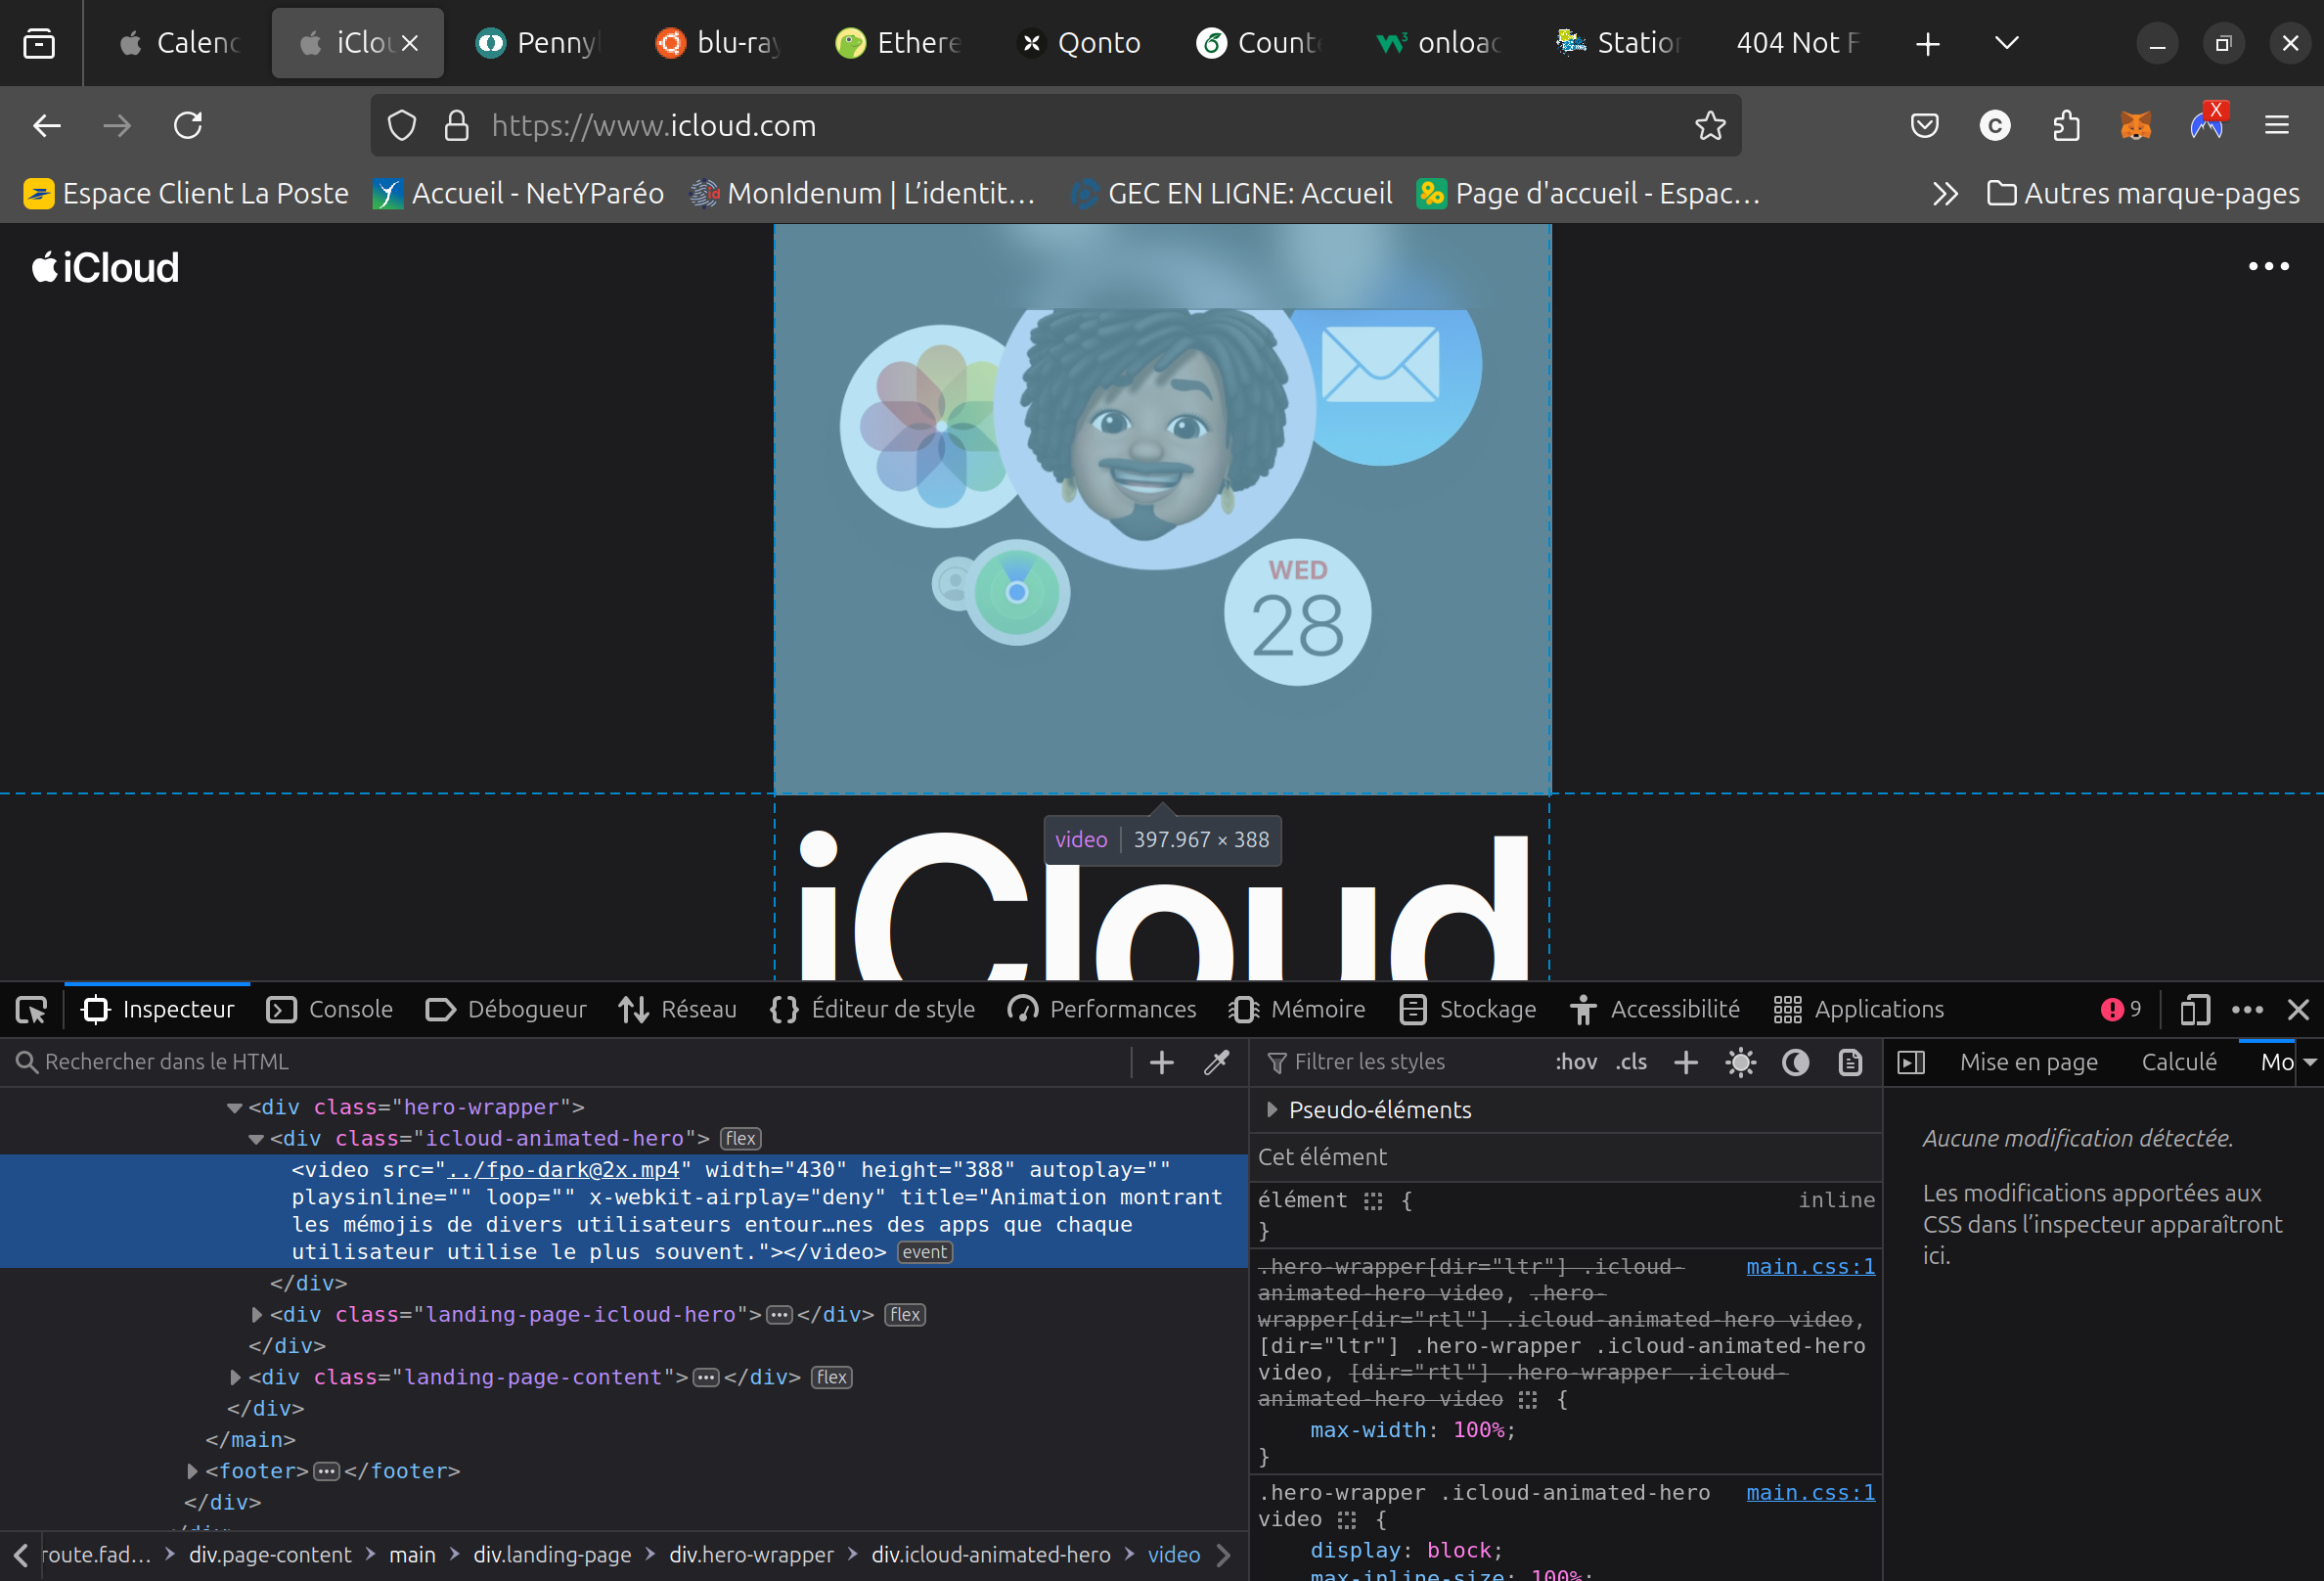
\includegraphics[width=7cm]{image/inspector-highlight}
    \end{frame}

    \begin{frame}{Les bases du débug}{Inspection du HTML}
        Exercice \execcounterdispinc{}~:
        \bigbreak
        \begin{itemize}
            \item Inspecter la page \url{https://www.icloud.com/calendar/}.
            \item Trouver la classe du texte \textit{Organisez votre temps avec Calendrier iCloud. Vos calendriers sont toujours à jour sur n’importe quel appareil et sur le Web.}.
            \item Trouver la police de caractère de cette classe.
            \item Modifier la police de caractère de cette classe pour \textit{Comic Sans MS} et vérifier la prise en compte de la modification.
        \end{itemize}
        \bigbreak
        \centering
        
\includegraphics[width=3cm]{image/intelligence}
    \end{frame}

    \begin{frame}{Les bases du débug}{La console}
        La console est dédiée au JS, elle permet d'écrire du JS ou d'appeler du JS déjà connu de la page.
        \bigbreak
        \centering
        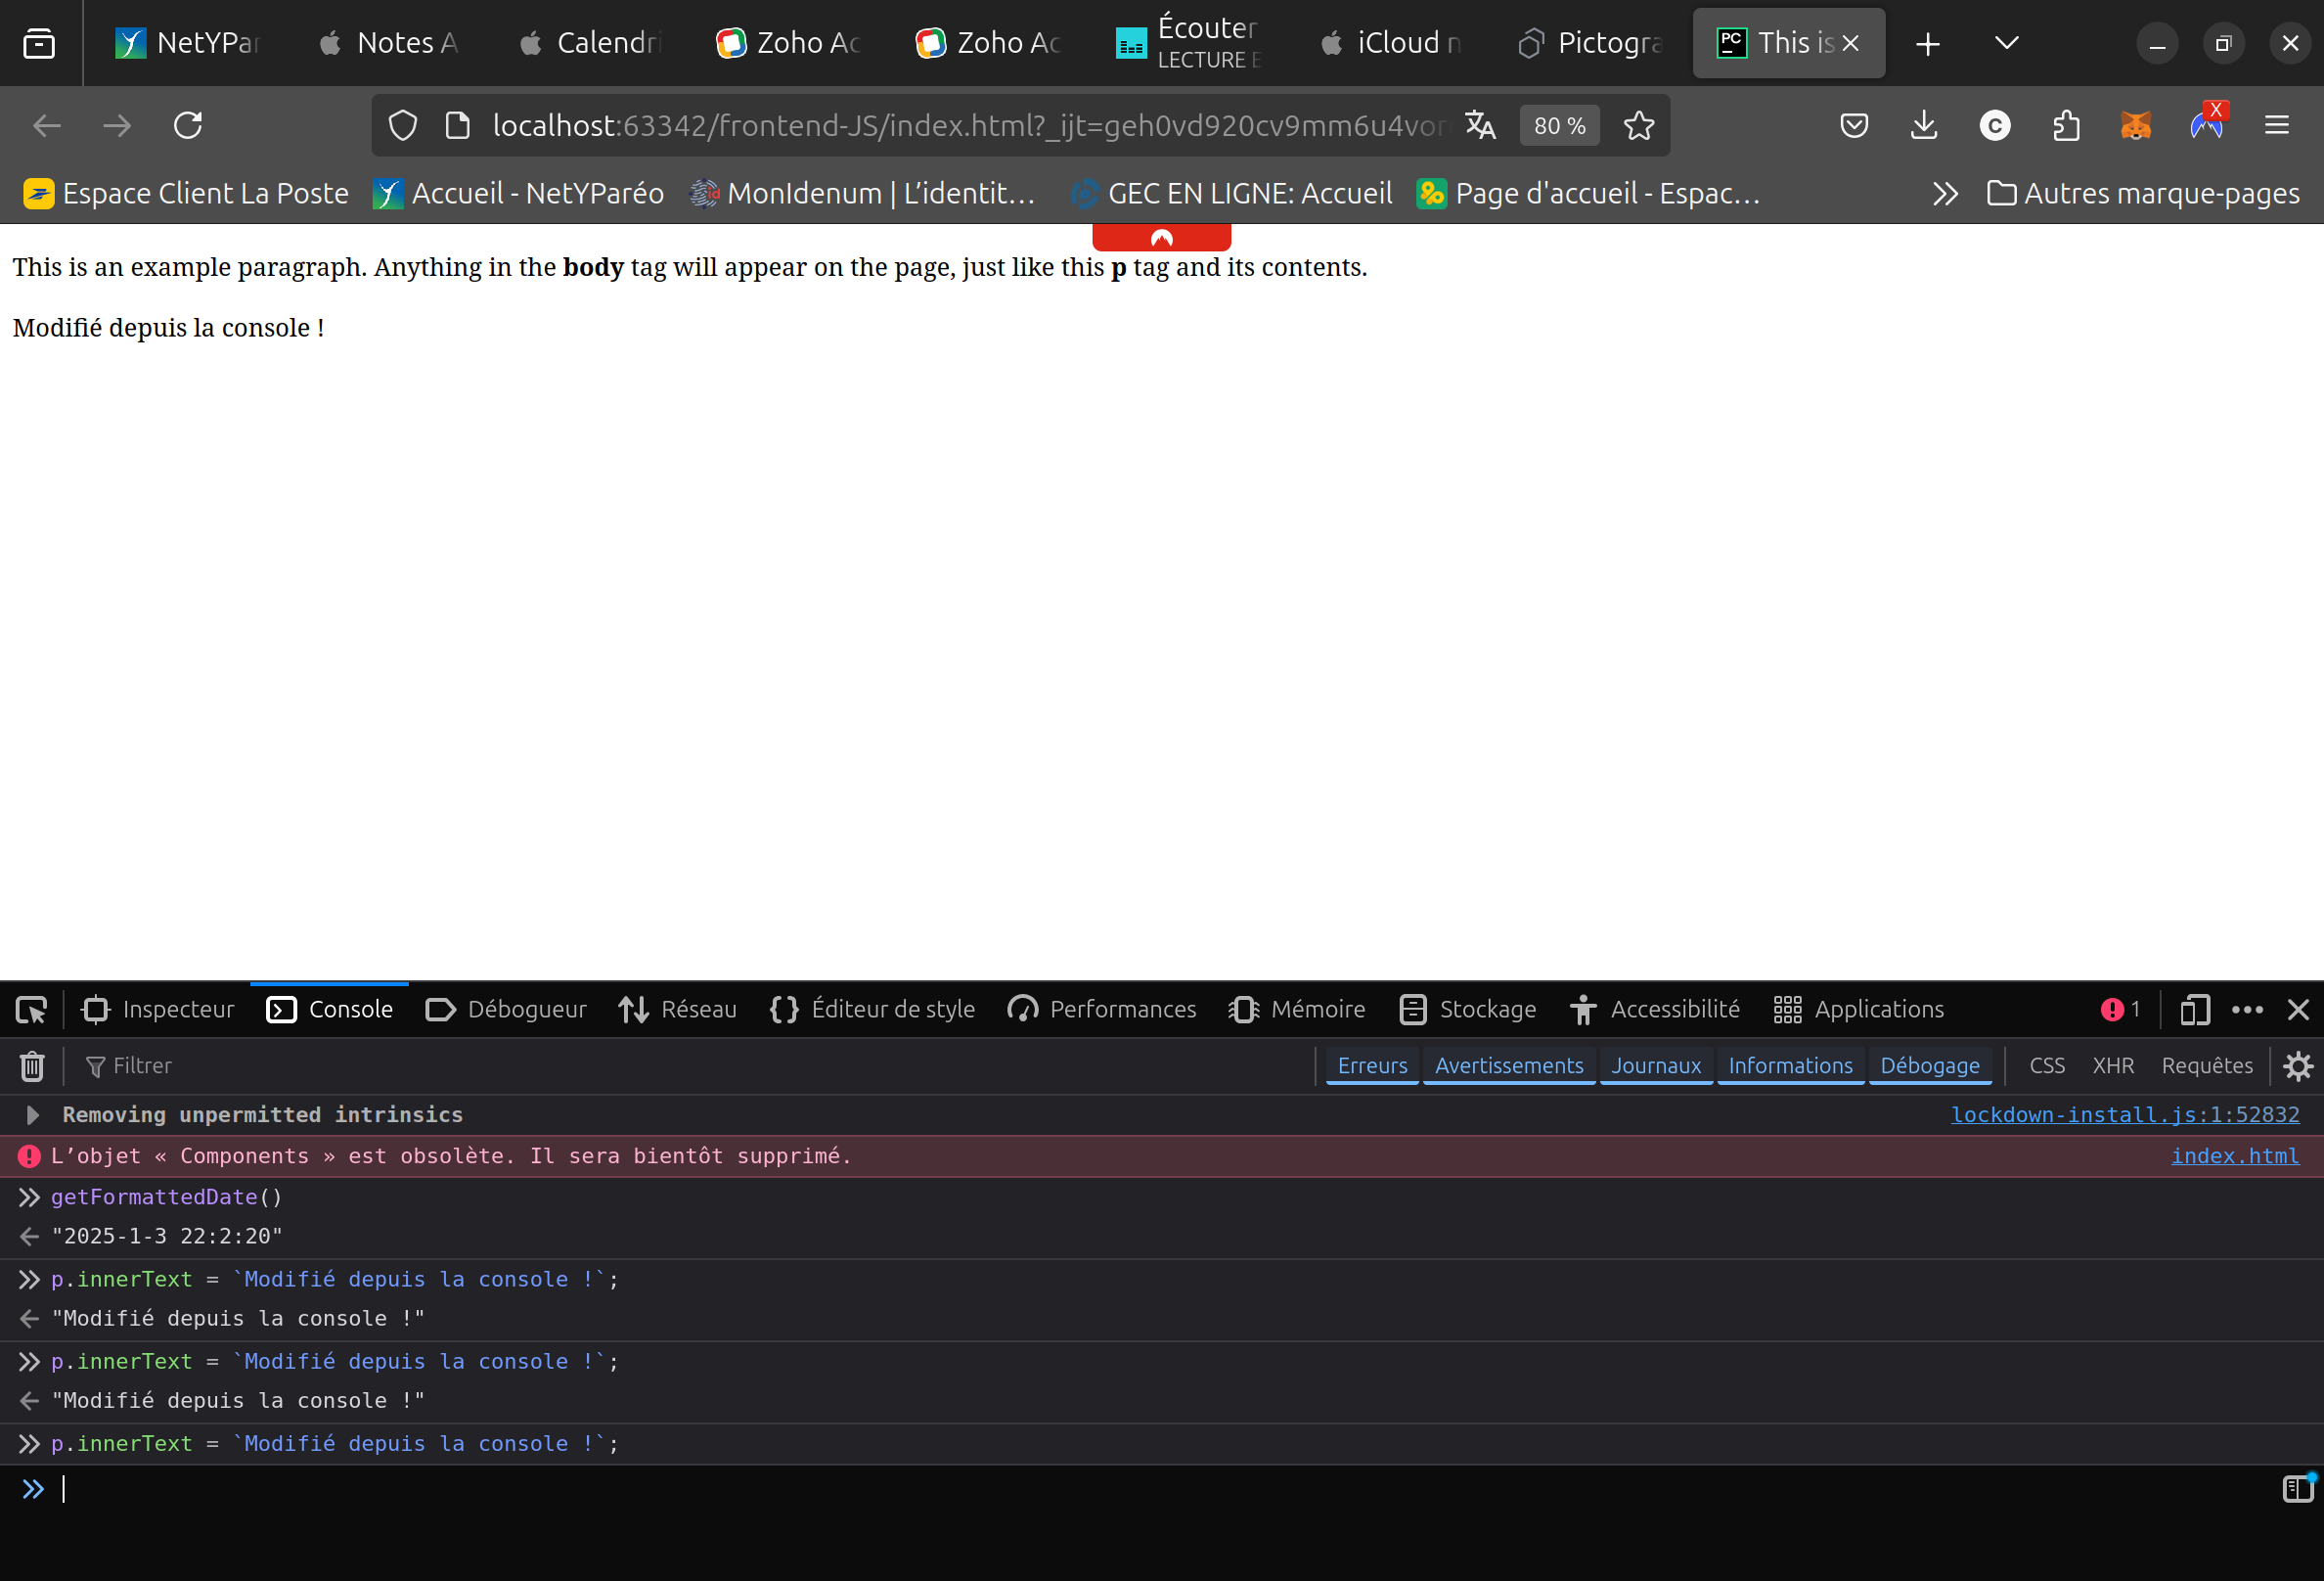
\includegraphics[width=8cm]{image/js-in-console}
        \bigbreak
        \flushleft
        Expliquer le comportement ci-dessus.
    \end{frame}

    \begin{frame}{Les bases du débug}{La console}
        Elle affiche (\textit{log}) les éventuels messages de warning, info, erreur lors de l'exécution et les erreurs de syntaxe.
        \bigbreak
        \centering
        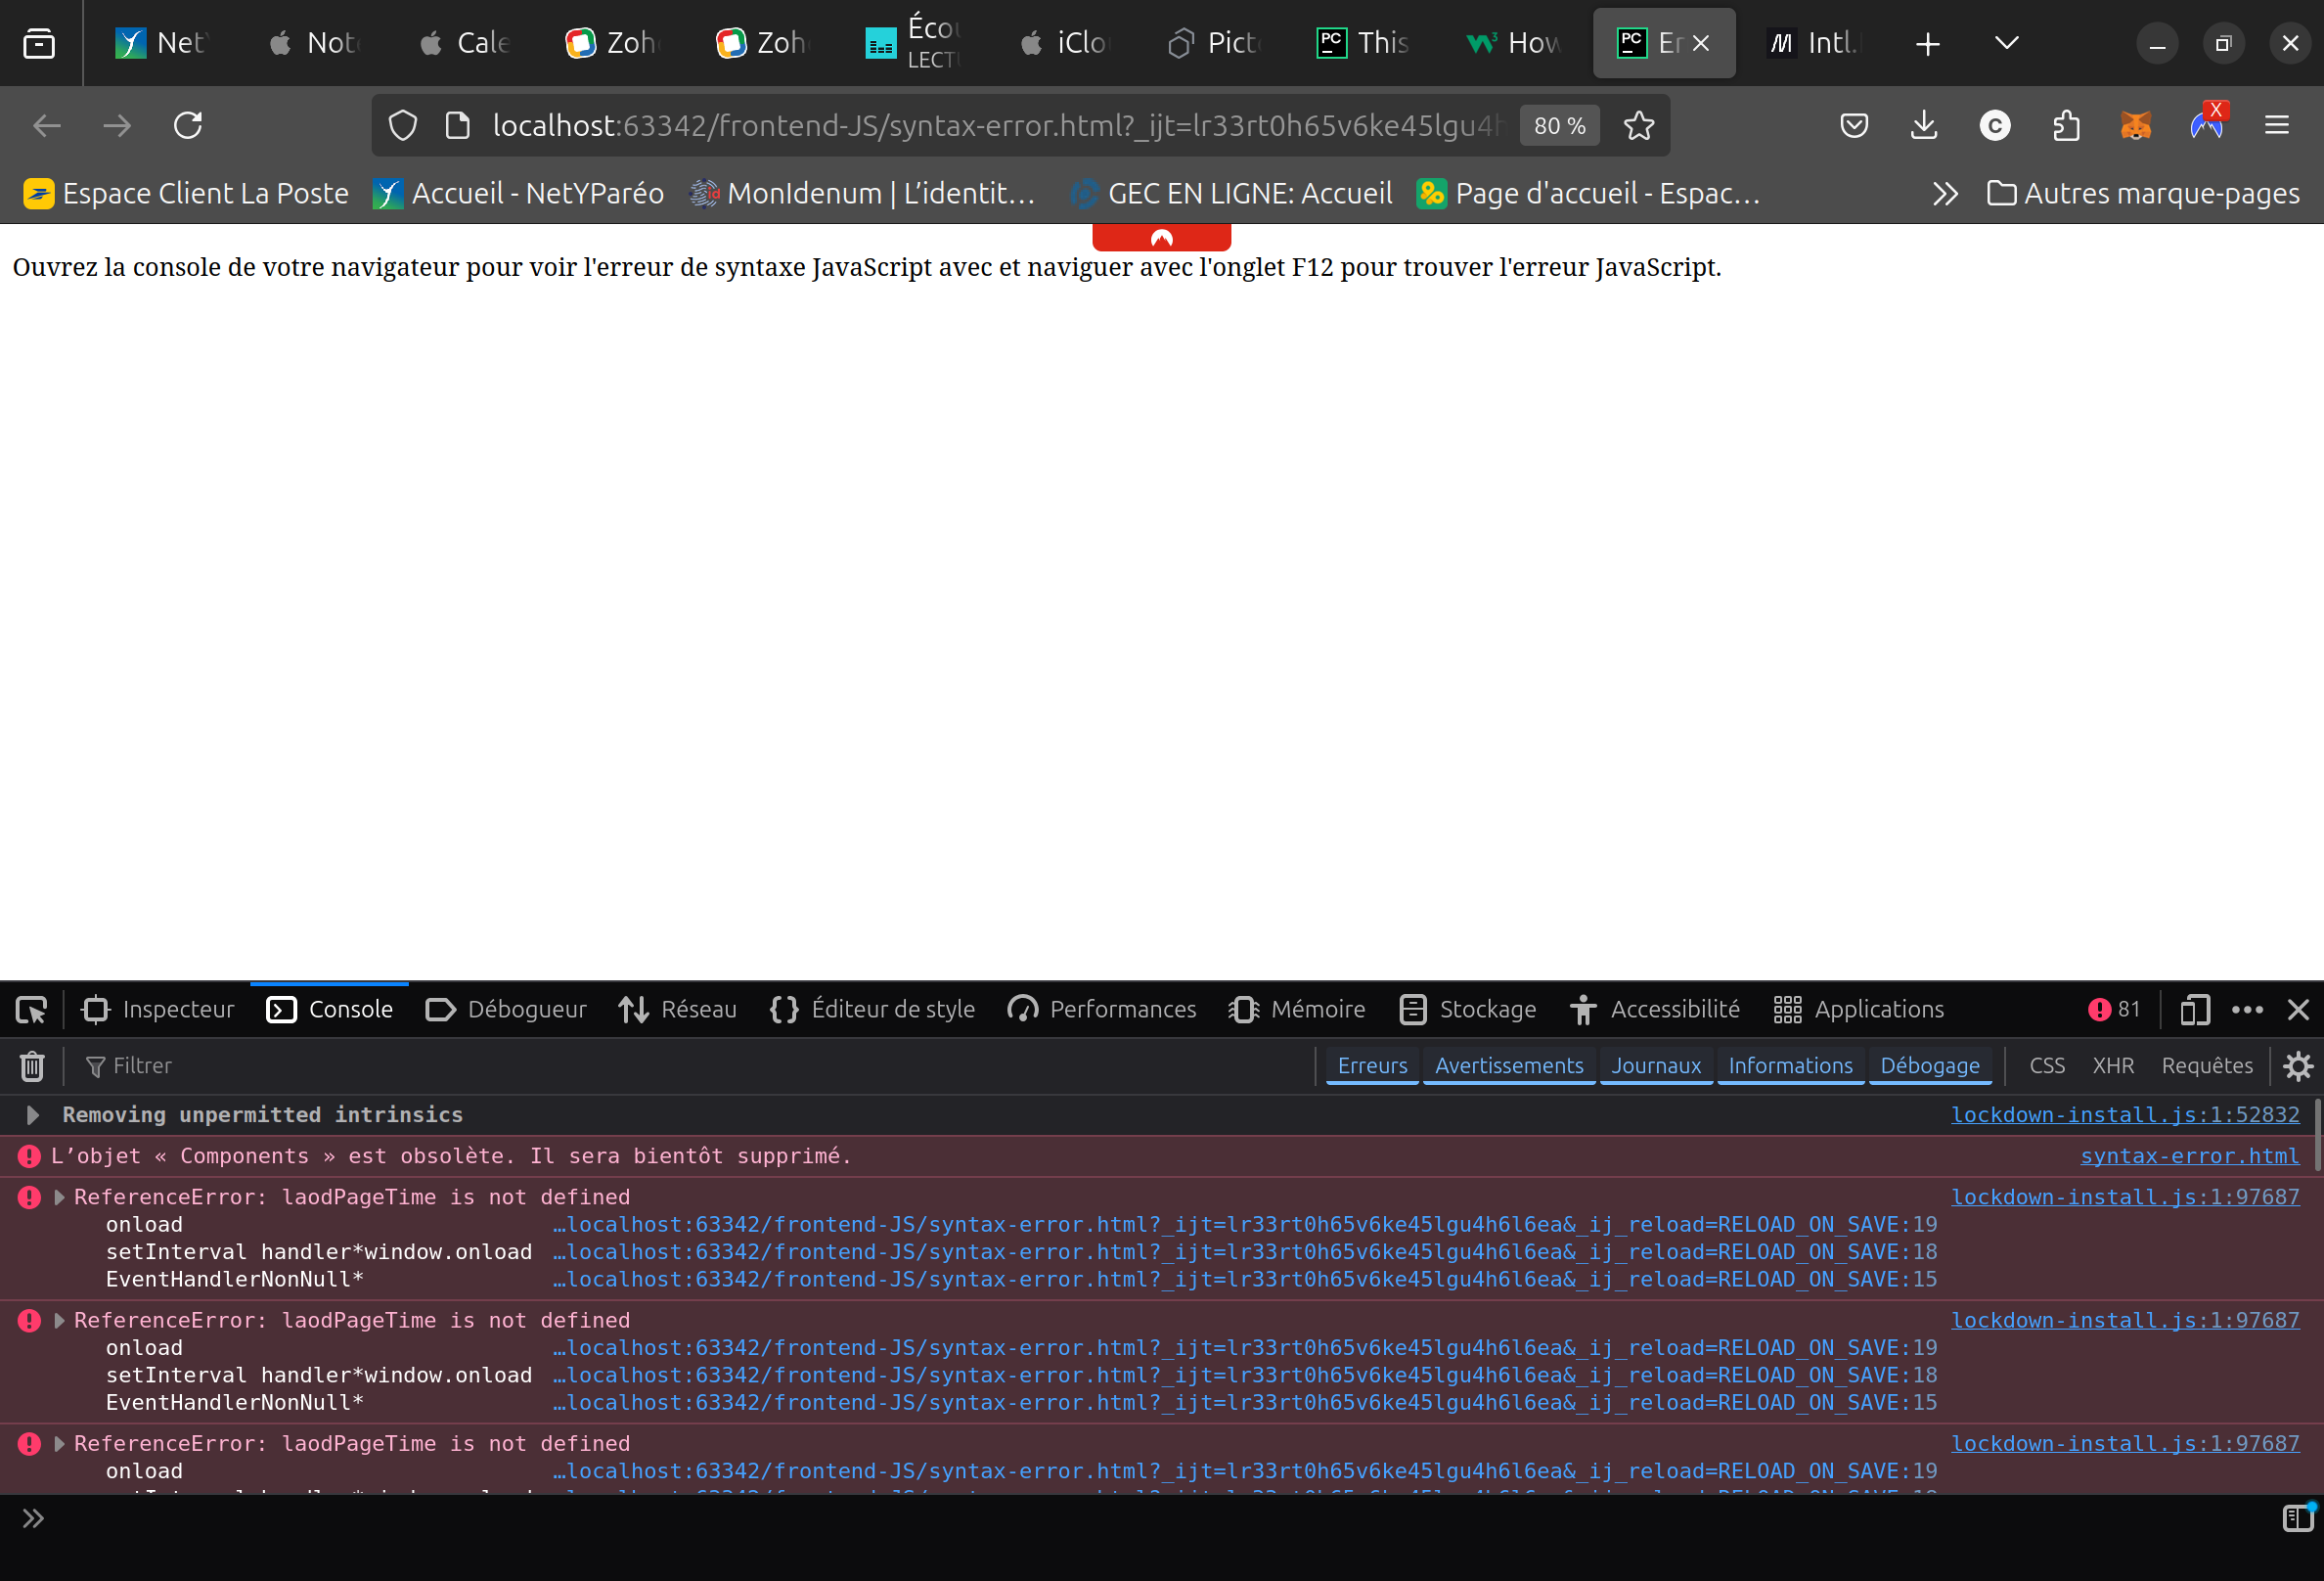
\includegraphics[width=7cm]{image/js-console-error-message}
        \flushleft
        On voit ici le parcours de l'interpréteur jusqu'à l'erreur en commençant par le dernier des appels.
    \end{frame}

    \begin{frame}{Les bases du débug}{La console}
        En cliquant sur le lien, on arrive sur le code source de l'erreur dans le débogueur.
        \bigbreak
        \centering
        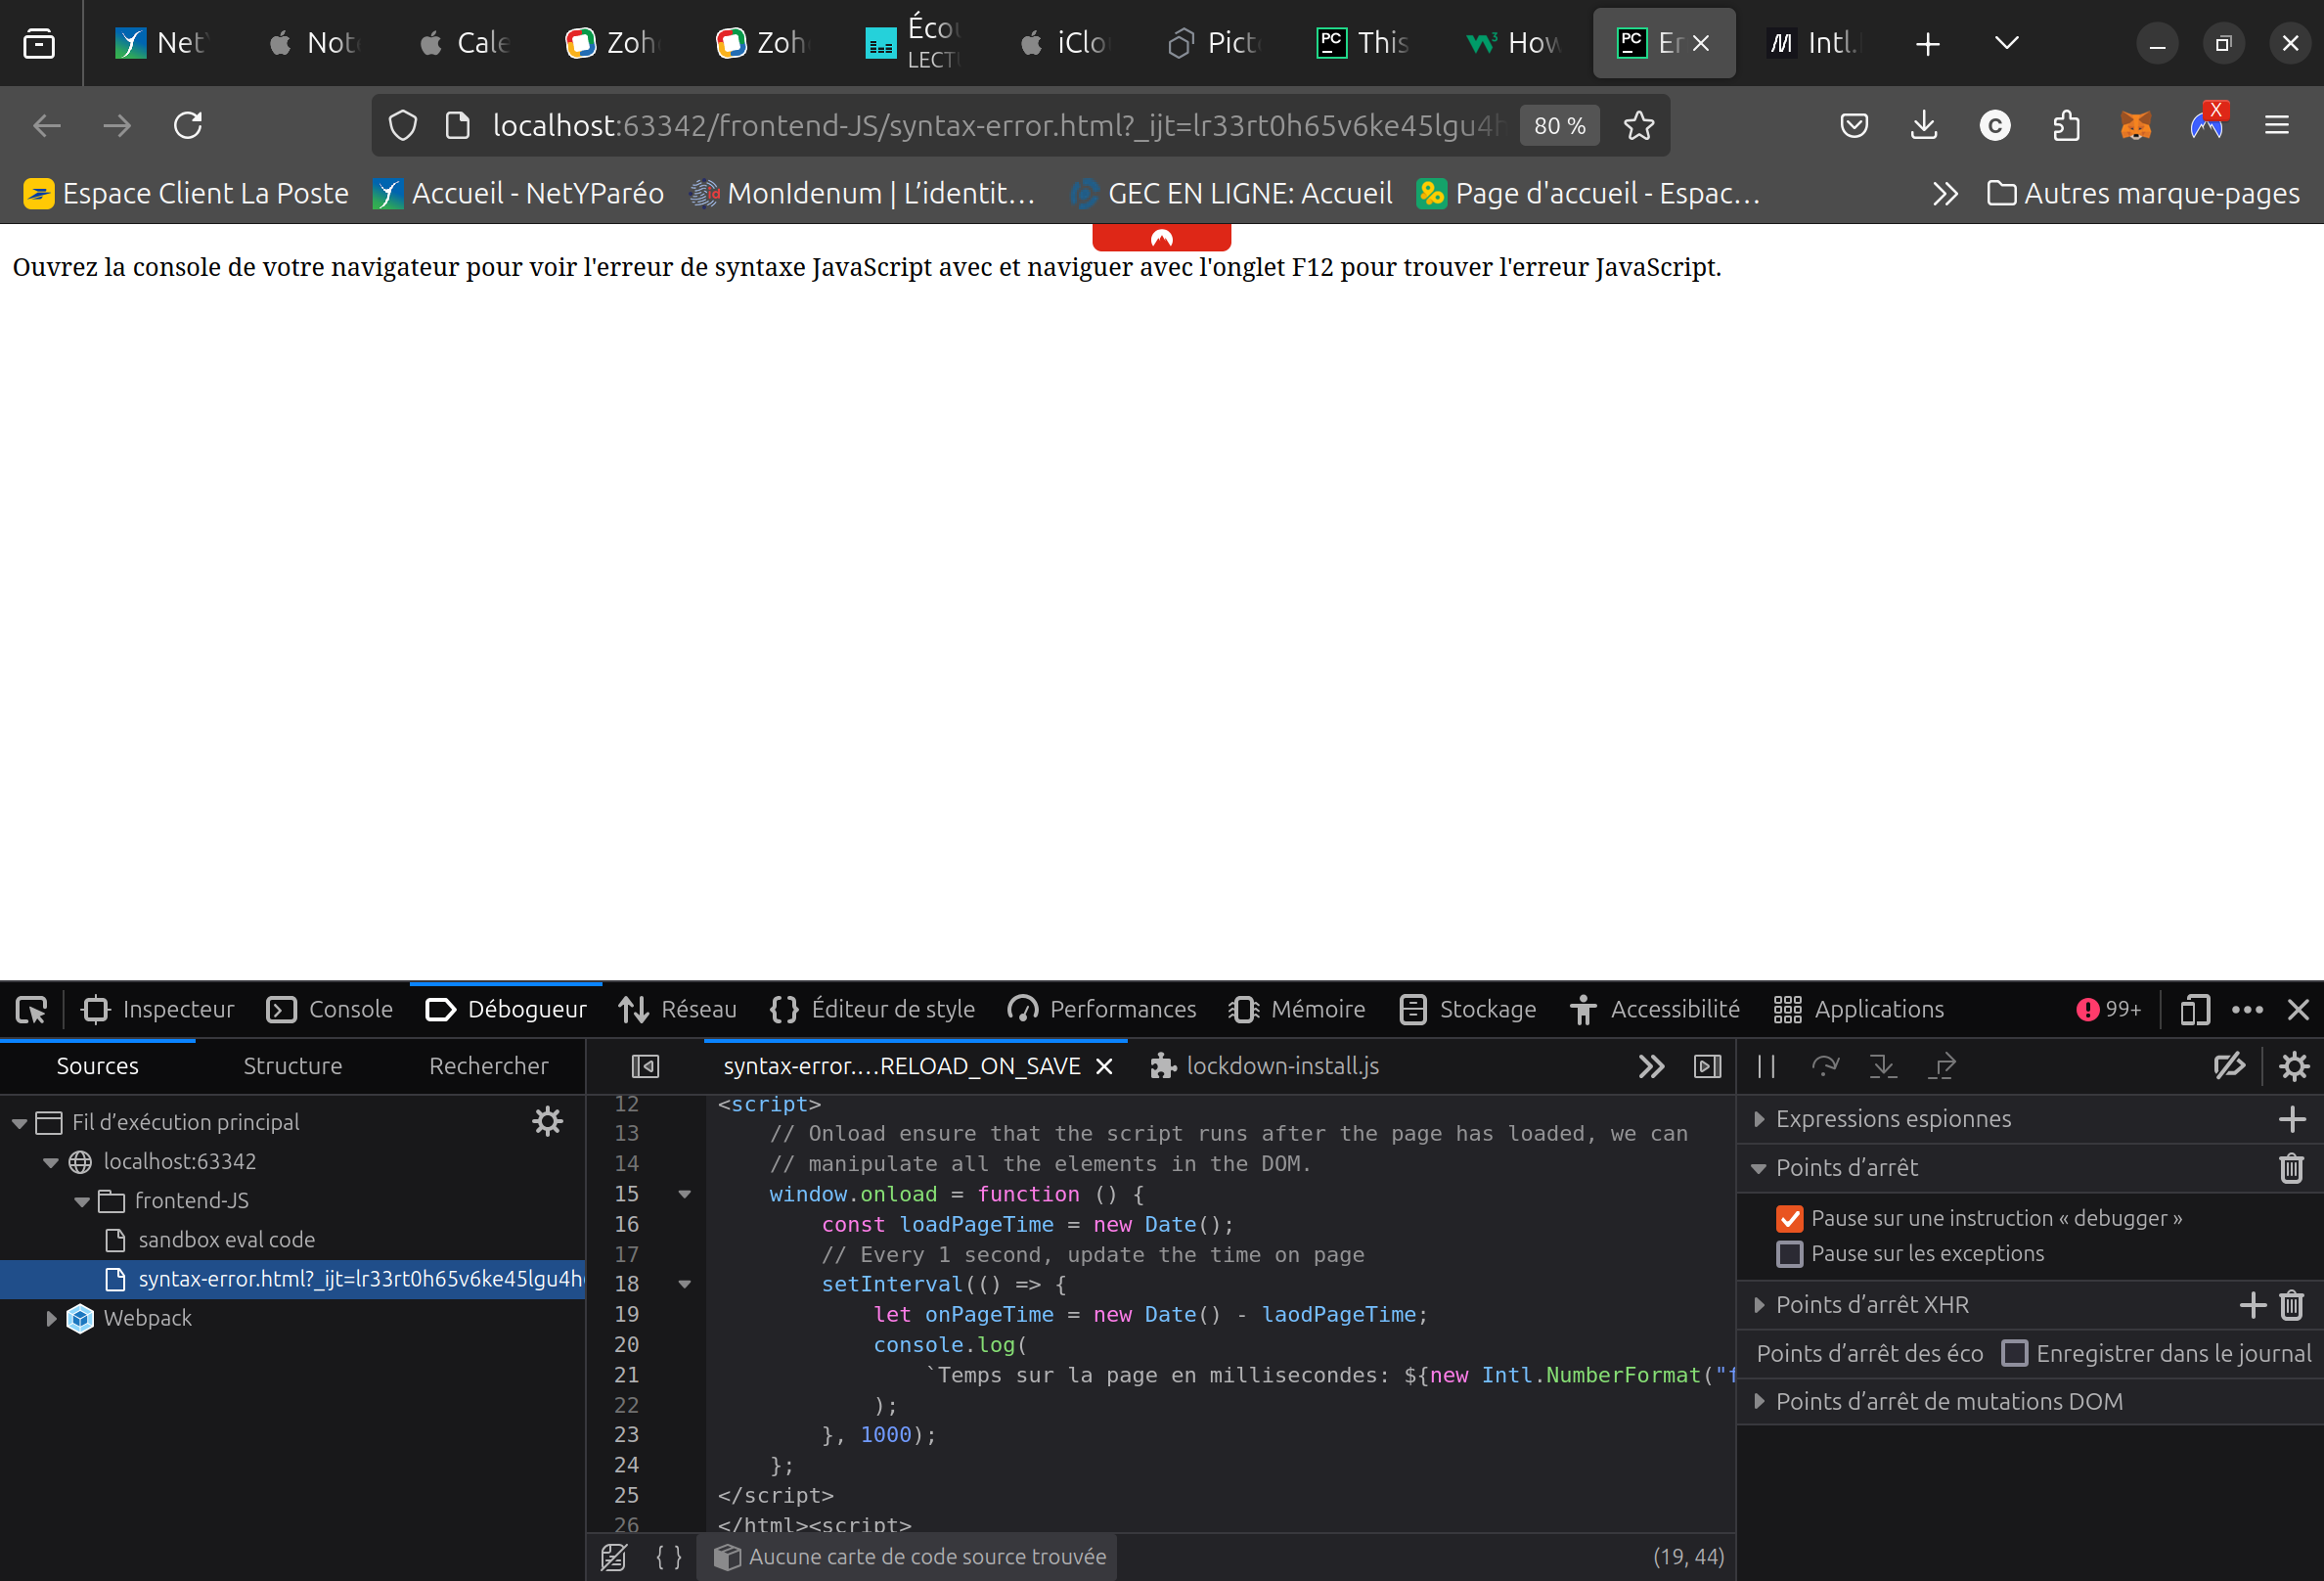
\includegraphics[width=9cm]{image/js-console-error-code}
    \end{frame}

    \begin{frame}{Les bases du débug}{Le débogueur}
        Le débogueur est, lui aussi, dédiée au JS, elle permet~:
        \begin{itemize}
            \item De lire le JS de la page.
            \item De mettre des points d'arrêt (\textit{breakpoints}) pour arrêter l'exécution du code.
            \item De naviguer dans le code, de pas en pas, de sauter des fonctions.
            \item De voir les valeurs des variables à un instant donné.
            \item De voir la pile d'appel des fonctions.
        \end{itemize}
    \end{frame}

    \begin{frame}{Les bases du débug}{Le débogueur}
        \bigbreak
        \centering
        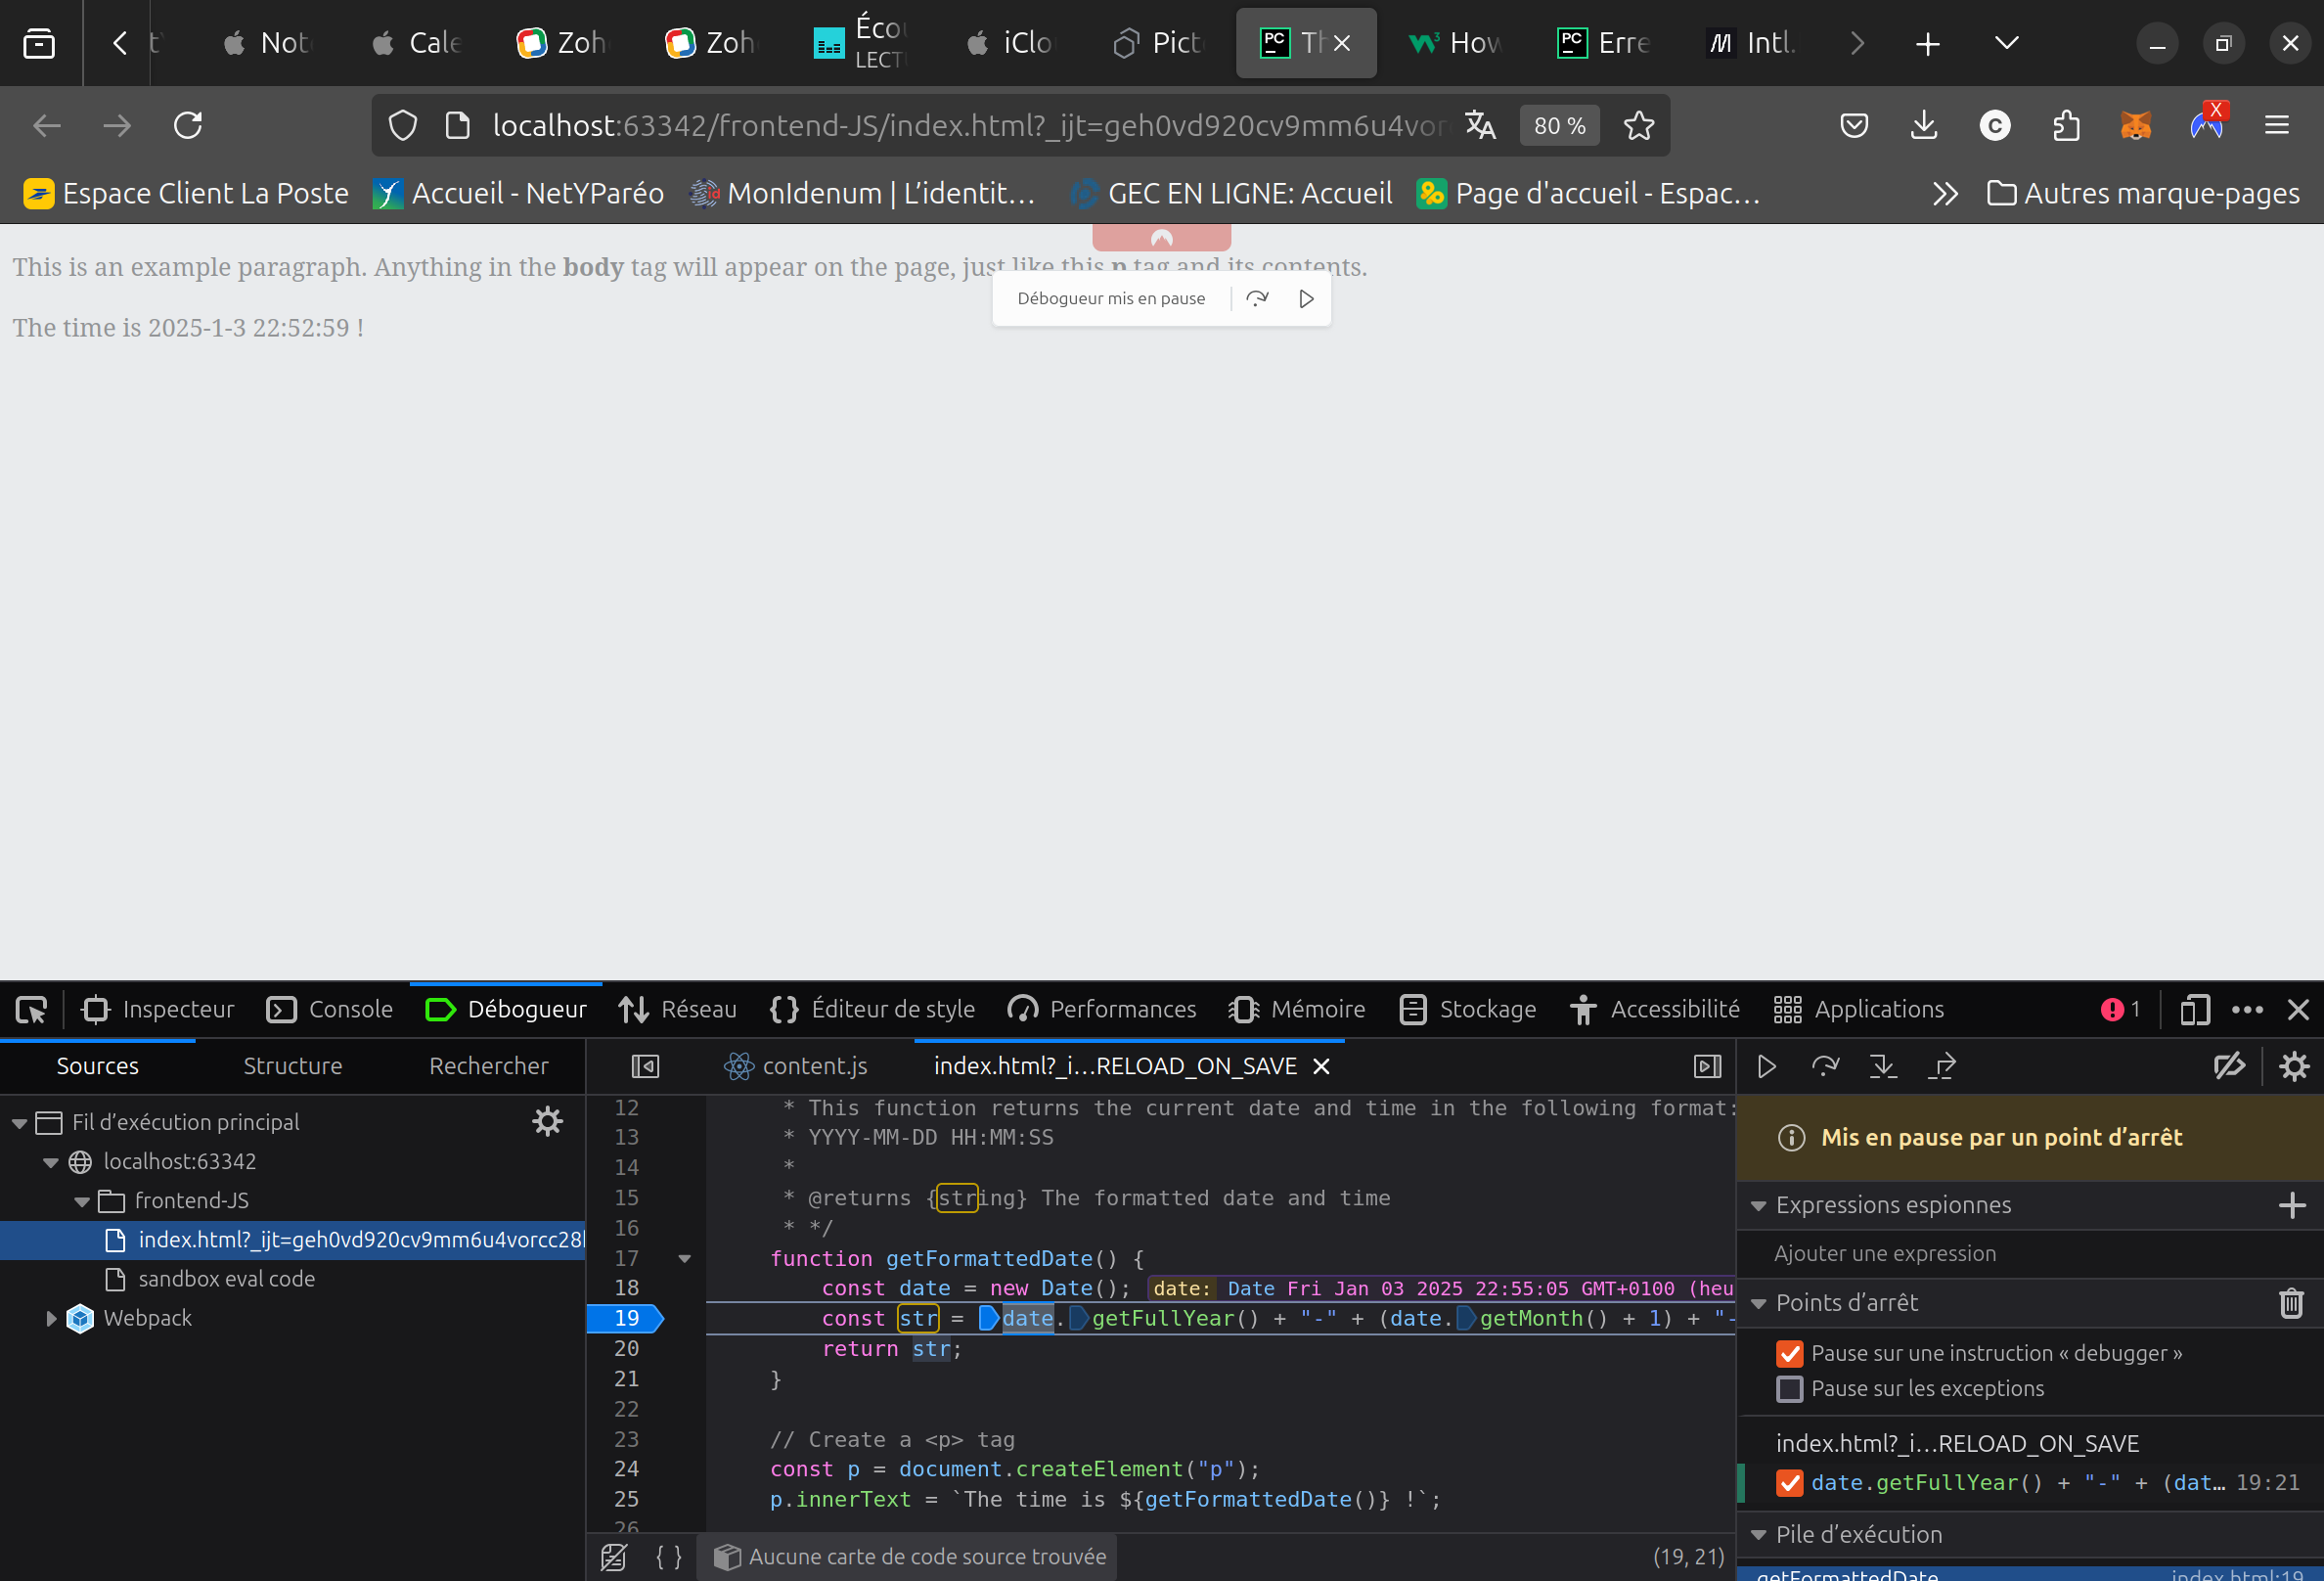
\includegraphics[width=10cm]{image/js-debugger}
    \end{frame}

    \begin{frame}{Les bases du débug}{Console et débogueur}
        Exercice \execcounterdispinc{}~:
        \begin{itemize}
            \item Naviguer à l'adresse \url{http://0.0.0.0/syntax-error.html}.
            \item Ouvrir la console.
            \item Cliquer sur le dernier appel pour aller au plantage
            \item Lire le code dans le débuggeur pour trouver l'erreur.
            \item Corriger l'erreur dans le code source et recharger la page.
        \end{itemize}
        \bigbreak
        \centering
        
\includegraphics[width=3cm]{image/intelligence}
    \end{frame}

    \begin{frame}{Les bases du débug}{Débogueur}
        Exercice \execcounterdispinc{}~:
        \begin{itemize}
            \item Naviguer à l'adresse \url{http://0.0.0.0/}.
            \item Ouvrir la débuggeur.
            \item Ajouter un point d'arrêt dans la fonction \lstinline{getFormattedDate}.
            \item Observer ce qui se passe.
            \item Faire du pas à pas pour comprendre le code.
        \end{itemize}
        \bigbreak
        \centering
        
\includegraphics[width=3cm]{image/intelligence}
    \end{frame}


    \section{Le langage JavaScript}\label{sec:js-lang}
    \begin{frame}{JavaScript}{L'historique\footnote{\label{mozilla-js}Une réintroduction à JavaScript, \url{https://developer.mozilla.org/fr/docs/Web/JavaScript/Language_overview}}}
        \begin{itemize}
            \item Créé en 1995 par Brendan Eich chez Netscape.
            \item En 1996, Java est très populaire et Netscape veut surfer sur la vague et renomme le langage appelé LiveScript en JavaScript.
            \item Standardisé par l'ECMA (European Computer Manufacturers Association) en 1997.
            \item Le standard est l'ECMAScript.
            \item La version actuelle implémentée dans les navigateurs se base sur le standard ES6 de 2015/2016.
            \item Les navigateurs implémentent des versions différentes de l'ES.
            \item JS est partout dans le backend ou programmation système avec Bun ou Node.js, pour le scripting de NoSQL comme CouchDB ou MongoDB, dans les PDF, \textit{etc}.
        \end{itemize}
    \end{frame}

    \begin{frame}{L'écosystème JavaScript}{Un langage interprété}
        \centering
        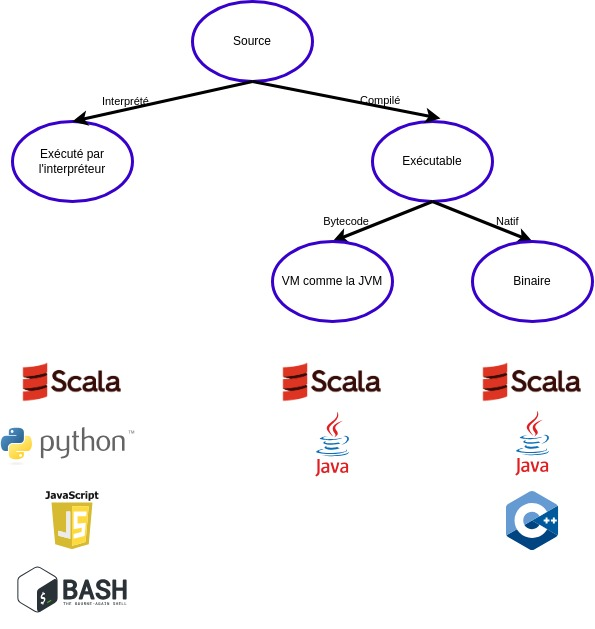
\includegraphics[width=7cm]{image/code-inter-vs-compiled}
    \end{frame}

    \begin{frame}{L'écosystème JavaScript}{Un langage interprété}
        \begin{small}
            De nombreux interpréteurs JavaScript existent dans les navigateurs, mais aussi en dehors~:
            \begin{itemize}
                \item \textbf{V8}, le moteur JavaScript de Chrome.
                \item \textbf{Node.js}, un interpréteur JavaScript côté serveur basé sur V8.
                \item \textbf{Deno}, un interpréteur JavaScript côté serveur basé sur V8, écrit en Rust par le développeur Node.js, il devrait lui succéder.
                \item \textbf{JavaScriptCore}, le moteur JavaScript de Safari.
                \item \textbf{SpiderMonkey}, le moteur JavaScript de Firefox.
                \item \textbf{Bun}, un environnement d'exécution plus rapide que Node.js et Deno\footnote{\label{bun}Bun is a fast JavaScript, \url{https://bun.sh/}}.
                \item \textbf{CouchDB}, une base de données NoSQL qui utilise JavaScript pour les requêtes dans sa version ES6 grâce à son binding avec SpiderMonkey, \footnote{The Road to CouchDB 3.0: Update to JavaScript Engine, \url{https://blog.couchdb.org/2020/02/26/the-road-to-couchdb-3-0-update-to-javascript-engine/}}.
                \item \textit{Many more}.
            \end{itemize}
        \end{small}
    \end{frame}

    \begin{frame}{L'écosystème JavaScript}{Les limites de notre cours}
        Sachant que ce cours s'appelle \textit{JavaScript Frontend}, dans quel(s) partie(s) de l'écosystème JavaScript allons-nous nous programmer~?
        \bigbreak
        \centering
        
\includegraphics[width=3cm]{image/intelligence}
        \pause
        \bigbreak
        Du code JavaScript exécuté dans le navigateur, donc du JavaScript côté client.
    \end{frame}

    \begin{frame}{JavaScript dans le navigateur}{Les limites}
        Il existe de nombreuses limites à ce que peut faire le JavaScript dans le navigateur, principalement pour des raisons de sécurité~:
        \begin{itemize}
            \item Pas d'accès au système de fichiers, A.K.A. \textit{File System}, le disque dur.
            \item Capacités réseau limitées, seule une partie du protocole HTTP et le protocole WebSocket.
            Tout ce qui est protocole de bas niveau comme TCP, UDP, \textit{etc} est interdit.
            Il ne peut être que client, pas serveur.
            \item Le stockage de donnée se fait dans le navigateur, dans les cookies, le \textit{localStorage}, le \textit{sessionStorage} principalement.
            \item Pas d'accès à l'OS, donc pas de gestion de processus, tout est isolé dans le navigateur.
        \end{itemize}
    \end{frame}

    \begin{frame}{JavaScript dans le navigateur}{Les spécificités}
        \begin{scriptsize}
            Les spécificités du navigateur sont ses 2 A.P.I. (Application Programming Interface)~:
            \begin{itemize}
                \item Le DOM (Document Object Model)\footnote{Référence du DOM, \url{https://developer.mozilla.org/fr/docs/Web/API/Document_Object_Model}}, qui permet de manipuler le contenu de la page dans les langages de balises HTML, XML, SVG.
                \item Le BOM (Browser Object Model)\footnote{Introduction au Browser Object Model (BOM) et à l’objet Window, \url{https://www.pierre-giraud.com/javascript-apprendre-coder-cours/browser-object-model-window/\#google_vignette}}, qui permet de manipuler le navigateur et ses fenêtres (\lstinline{window})~:
                \begin{itemize}
                    \begin{scriptsize}
                        \item L’objet \lstinline{Navigator} qui représente l’état et l’identité du navigateur et qu’on va utiliser avec l’API Geolocation.
                        \item L’objet \lstinline{History} qui permet de manipuler l’historique de navigation du navigateur.
                        \item L’objet \lstinline{Location} qui fournit des informations relatives à l’URL de la page courante.
                        \item L’objet \lstinline{Screen} qui nous permet d’examiner les propriétés de l’écran qui affiche la fenêtre courante.
                        \item L’objet \lstinline{Document} et le DOM dans son ensemble que nous étudierons en détail dans la suite.
                    \end{scriptsize}
                \end{itemize}
            \end{itemize}
        \end{scriptsize}
    \end{frame}

    \begin{frame}{JavaScript dans le navigateur}{Les prérequis}
        Pour utiliser une API, quelle qu'elle soit, quel que soit le langage, il faut d'abord maîtriser les bases de ce dernier.
        \bigbreak
        Les bases de JS que nous allons couvrir ici sont les suivantes~:
        \begin{itemize}
            \item Les types
            \item La déclaration de variables
            \item Les structures de contrôle (\textit{control flow})
            \item La déclaration de fonctions
            \item Les objets
            \item Les méthodes built-in
            \item Les exceptions
        \end{itemize}
    \end{frame}

    \subsection{Installation de WebStorm}\label{subsec:installwebstorm}

    \begin{frame}{Développement d'un script}{Installation d'un IDE}
        Un IDE est un \textit{Integrated Development Environment}, un environnement de développement intégré, logiciel d'édition de texte dédié à la programmation.
        \bigbreak
        Les principaux environnements de développement en JS sont VS Code de Microsoft et WebStorm de JetBrains.

        WebStorm est gratuit pour les étudiants, vous pouvez avoir une licence en créant un compte avec votre adresse MDS~.
        \bigbreak
        \bigbreak
        \centering
        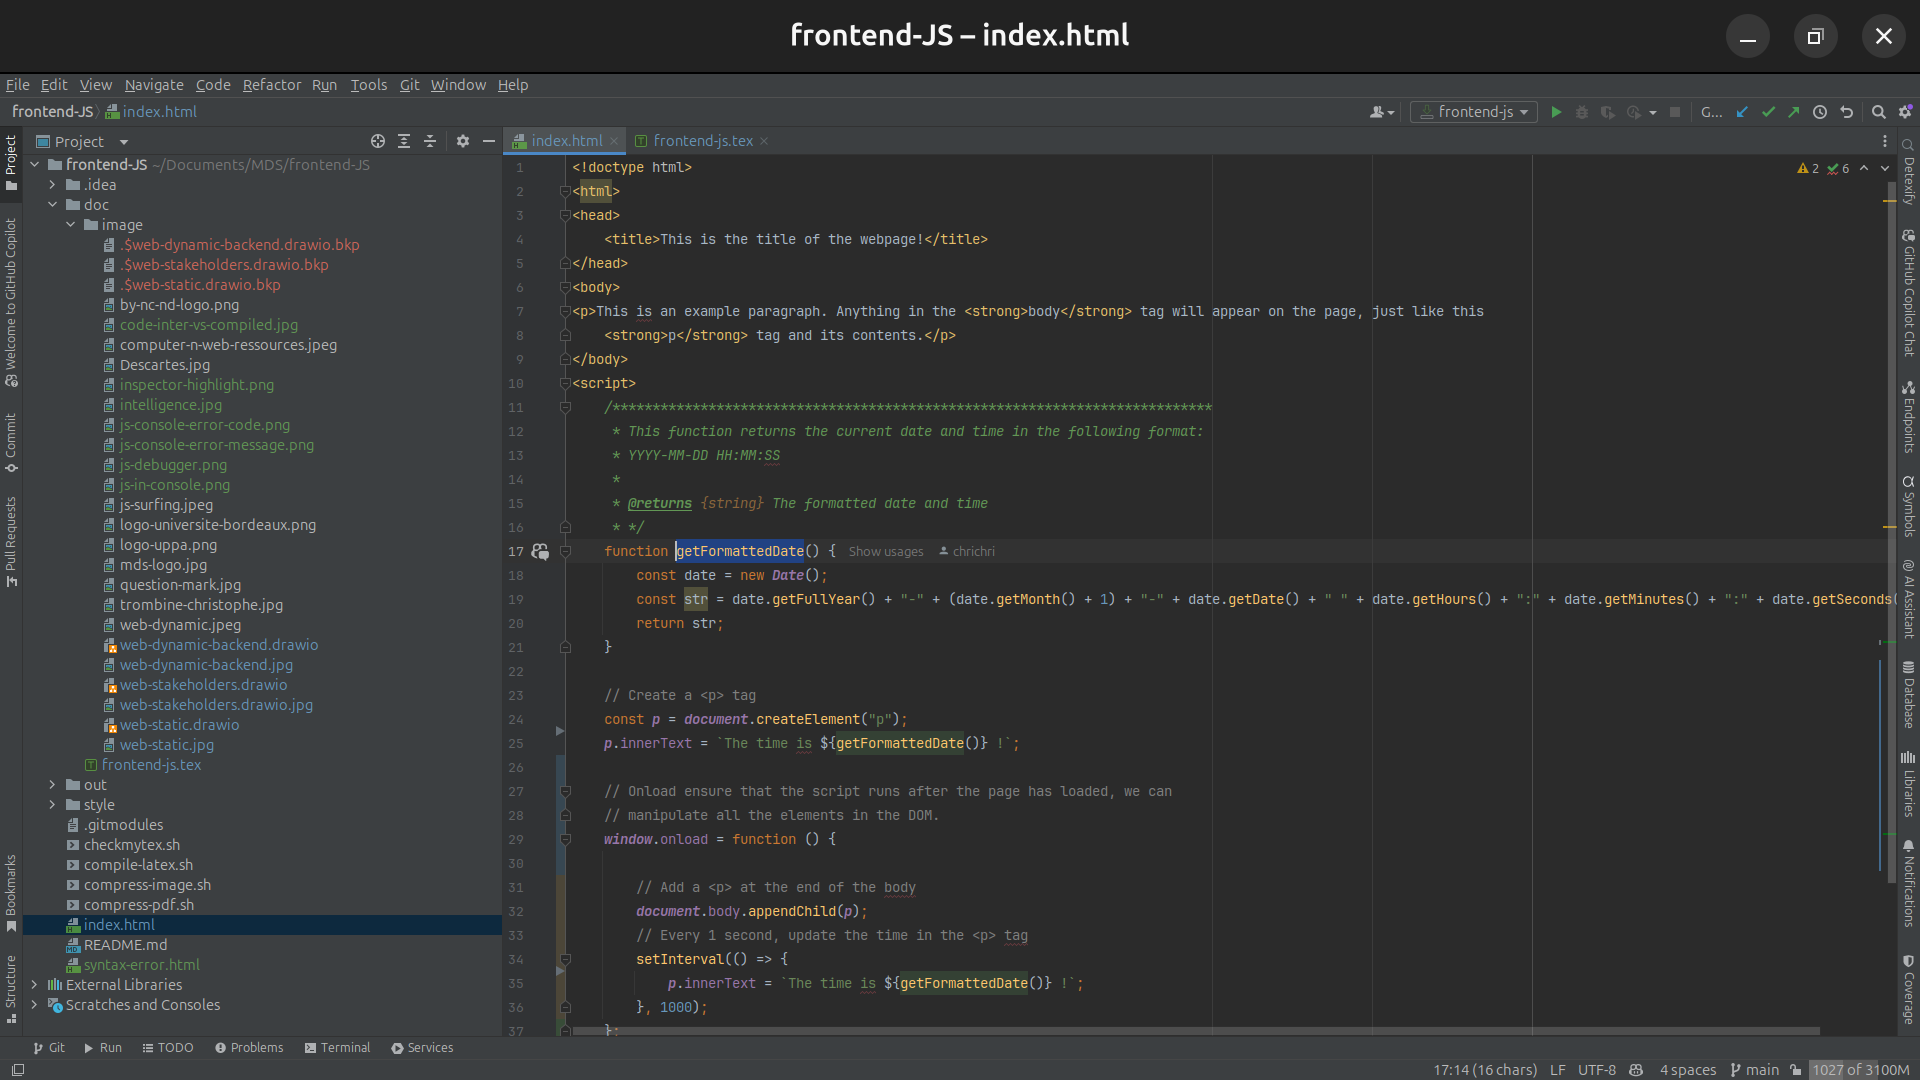
\includegraphics[width=6cm]{image/webstorm}
    \end{frame}

    \subsection{Initialisation du projet}\label{subsec:projectinit}

    \begin{frame}{Développement d'un script}{Mon premier script}
        \begin{itemize}
            \item Télécharger le code de ce cours sur GitHub \url{https://github.com/My-Digital-School-by-PapIT/frontend-JS}.
            \item Dézipper l'archive.
            \item Ouvrir le dossier avec WebStorm.
            \item Créer un fichier avec une extension comme \lstinline{variables-n-types.js} par exemple.
        \end{itemize}
        \bigbreak
        \centering
        
\includegraphics[width=3cm]{image/intelligence}
    \end{frame}


    \section{Licence CC}\label{sec:licence}

    \begin{frame}{Licence}{Licence Creative Commons}
        Support de cours sous licence Creative Commons BY-NC-ND~.
        \bigbreak
        Vous pouvez donc, partager, copier, distribuer le document.
        \bigbreak
        Attribution requise à PapIT SASU - Pas d’utilisation commerciale - Pas de modification
        \bigbreak
        \centering
        
\includegraphics[width=5cm]{image/by-nc-nd-logo}
    \end{frame}


\end{document}
